\documentclass[a4paper,11pt]{jarticle}
\usepackage{ics-thesis}
\usepackage{amssymb}
\usepackage[dvipdfmx]{graphicx}
\usepackage{subcaption}
\pagestyle{bachelorthesis}    % 卒論・規定の.styファイルを使う場合
%
\title{サイボーグインセクトによる迅速な被災者発見のための自己組織型移動制御手法の提案と評価}
\author{北浦 直}
\supervisor{若宮 直紀 教授}
\deadline{2019年2月12日}
%
\begin{document}
	\titlepage    % 規定の.styファイルを使う場合
	\abstract     % 規定の.styファイルを使う場合
	%%%%%%%%%%%%%%%%%%%%%
	% 内容梗概本文
	%%%%%%%%%%%%%%%%%%%%%
	\keyword
	%%%%%%%%%%%%%%%%%%%%%
	% キーワード
	%%%%%%%%%%%%%%%%%%%%%
	\tableofcontents    % 目次
	%
	%%%%%%%%%%%%%%%%%%%%%
	% 本文
	%%%%%%%%%%%%%%%%%%%%%
	%
	\section{はじめに}
	災害が起きた場合,倒壊した建物内に被災者が取り残されることが起こりうる.
	倒壊した建物内に捕らわれた被災者の探索において,現在は災害救助犬やスコープカメラなどの人間の能力を補助するような手法が広く使われている\cite{USR}.
	しかし,倒壊した建物内は狭い隙間であったり,アスベストやほこり,危険物の存在により人間や災害救助犬が入れないような環境である可能性がある\cite{environment}.
	また,救助活動の中で2次災害が起きてしまう事例も少なくない.
	そこで,現在の探索手法では探索できないような狭い空間を探索可能で,探索中の2次災害の危険性を低くすることができるサイボーグインセクトを用いた被災者探索の研究がなされている\cite{CyborgInsect}.

	サイボーグインセクトを被災者探索に活用するための研究としてCINEMa(Cyborg Insect Networks for Exploration and Mapping)があげられる\cite{CINEMa}.
	この研究の中では,サイボーグインセクトへ制御を与えて任意の方向へ向かわせたり,サイボーグインセクトが位置推定をするためのアルゴリズムの実験がされていたりする.
	しかし,CINEMaはがれきなどが散乱するような悪条件下における被災者探索に必要な構成要素の説明は行われているが,それらを用いて被災者探索を効率的に行うための制御手法などは提案されていない.
	つまり,群で探索しているにも拘らず複数個体がほぼ同一の場所を探索することで空間全体を探索するのにかかる時間が増加してしまう恐れがある.
	
	そこで,サイボーグインセクトの群れが効率的に空間全体を探索できるような制御を与えたい.
	しかし,救助者は倒壊した建物内の詳細な環境を知ることはできないため,救助者から細かい操作を行うことは不可能である.
	よって,サイボーグインセクト自身が得られる情報をもとに自律的に制御を行い空間探索を行う必要がある.
		
	また,自律的な制御アルゴリズムの1つであるフロッキングという手法がある.
	フロッキングとは,周囲の個体に対して,衝突回避,中心移動,方向調整の3つの動作をとることで複数個体が群れとなって動くようなアルゴリズムである\cite{flocks}.
	文献\cite{flockingsearch}のようにフロッキングを被災者探索に適用される研究が行われているが,フロッキングをサイボーグインセクトに適用して被災者探索を実現している研究はなされていない.
	また,レスキューロボットなどのフロッキング制御とは違い,サイボーグインセクトに与えるフロッキングの制御は生物に電気信号を流すためできるだけ頻度が低いことが望ましい.
	
	そこで,本研究ではCINEMaで提案されているようなサイボーグインセクトの群れに対するフロッキング制御手法の提案を行う.サイボーグインセクトのモデルと断続的な制御をシミュレーション上に実装し,制御されていない場合の探索と制御された場合の探索を比較する.ここでは,サイボーグインセクトに対する断続的なフロッキング制御でも探索にかかる時間の短縮ができることを確認する.
	
	以降,第\ref{sec:CyborgInsect}章では,本研究に用いるサイボーグインセクトに関する説明を行い,第\ref{sec:flocking}章でフロッキング動作の説明を行う.第\ref{sec:algorithm}章でサイボーグインセクトが制御をされていない場合の動作について述べ,第\ref{sec:control}でサイボーグインセクトへ与える制御について述べる.第\ref{sec:result}章では実験結果について述べる.第\ref{sec:last}章では本研究のまとめと今後の課題について述べる.
	\section{サイボーグインセクト}
	\label{sec:CyborgInsect}
	この章では,本研究で考えるサイボーグインセクトの概要と,サイボーグインセクトに取り付けられる機材,サイボーグインセクトに関する条件の説明を行う.
	
	サイボーグインセクトとは,文献\cite{CyborgInsect}で示されているような,機械を埋め込み人間が操作できるようにした昆虫に計器類を乗せて被災者探索を可能にしたものを指す.
	このサイボーグインセクトの特徴として,昆虫の移動能力がそのまま使えるため,壁や天井も移動できて,かつ狭い場所にも侵入可能という探索できない場所の少なさが挙げられる.
	また,同等な移動能力を持つレスキューロボットに比べると1匹当たりの値段が安く済むため,探索に使える群の数を多くできることも利点である.
	
	サイボーグインセクトには,神経刺激による移動制御,センシング,サイボーグインセクトの位置推定、および救助者や周りのサイボーグインセクトとの通信のための機材が乗せられている.
	
	サイボーグインセクトに対する制御は,壁で仕切られた迷路の指定された経路を通るなどの実験を通して,サイボーグインセクトの本来の動きによらず移動の制御操作ができることを示している\cite{CINEMa}.
	
	文献\cite{CINEMa}の中で,センシングのために様々なセンサをサイボーグインセクトに積載すると示されている.具体的に挙げられていたのは,3方向の加速度計,ジャイロスコープ,磁力計,指向性マイクと全指向性マイク,ブザーとスピーカー,赤外線検知器,ガス検知器がサイボーグンセクトへ取り付ける機材として挙げられていた.
	
	被災者のセンシングに関して,複数のマイクでの音の強度を比較することで音源方向の特定をしてサイボーグインセクトから見た被災者の方向を特定することができていた.
	また,サイボーグインセクトに取り付けられたマイクとスピーカーを利用することによって,サイボーグインセクト自身の位置推定を行っていた.
	
	今研究では,神経刺激による移動制御は十分に可能として考える.被災者や障害物のセンシングは,半径2m以内ならできると考え,距離精度は10cm単位,角度の精度は10度単位として考える.
	また,サイボーグインセクト同士の通信可能範囲は5mとする.
	

	\section{フロッキング}
	\label{sec:flocking}
	この章では,フロッキングについて説明する.
	
	フロッキングとは,自然界の鳥や魚の群れで見られるような,複数の個体が同じ目標に向かい連動して動くような行動である.
	この自然界で見られる行動を限定された範囲のセンシング能力とコミュニケーションにより再現したモデルが知られている.
	文献\cite{steering}では衝突回避,中心移動,方向調整の3つの動作によりフロッキングのモデル化を行っている.それぞれの動きは図\ref{fig:flocking}のようにあらわされる.
	
	\begin{figure}
		\begin{minipage}{0.3\linewidth}
			\centering
			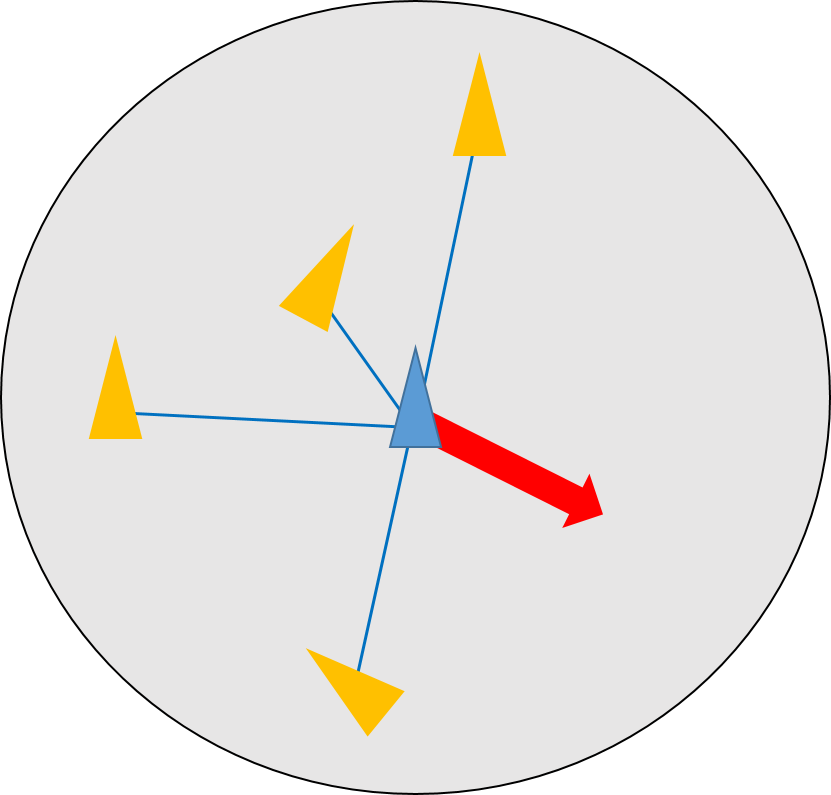
\includegraphics[width=0.9\linewidth]{png/separation.png}
			\subcaption{衝突回避}
		\end{minipage}
		\begin{minipage}{0.3\linewidth}
			\centering
			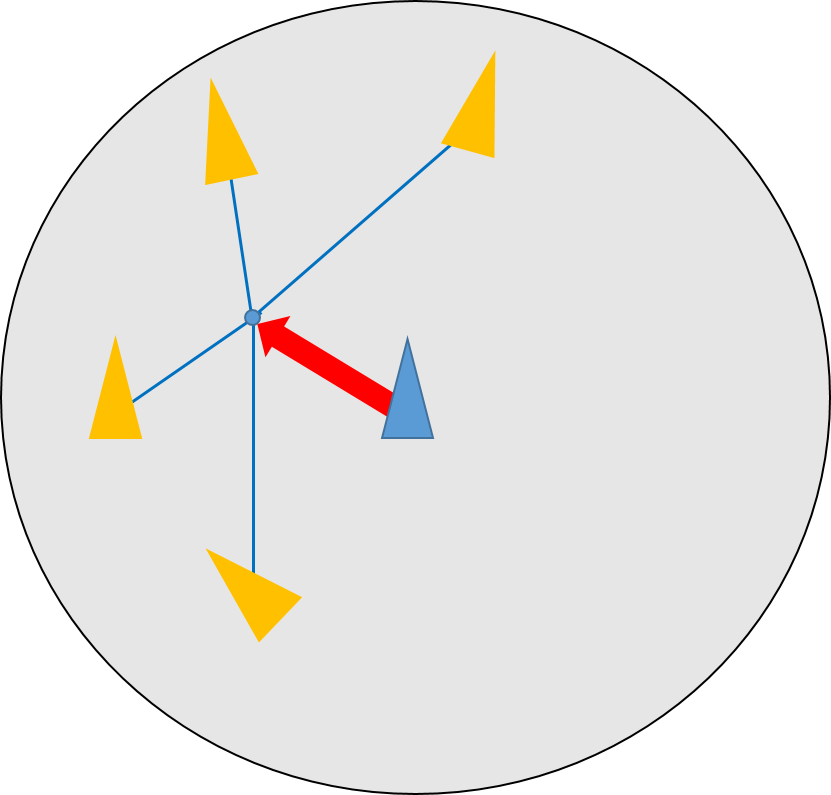
\includegraphics[width=0.9\linewidth]{png/cohesion.png}
			\subcaption{中心移動}
		\end{minipage}
		\begin{minipage}{0.3\linewidth}
			\centering
			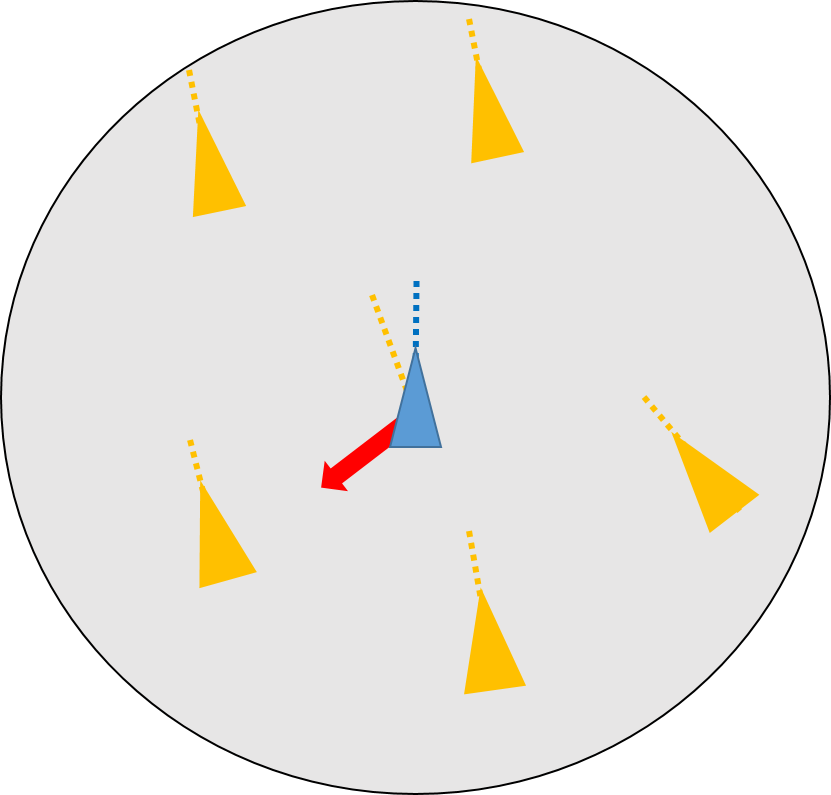
\includegraphics[width=0.9\linewidth]{png/alighnment.png}
			\subcaption{方向調整}
		\end{minipage}
		\caption[フロッキング]{フロッキングの動作}
		\label{fig:flocking}
	\end{figure}
	
	衝突回避の動作により,フロッキングを行っている個体群はそれぞれの距離を一定以上に保つことができる.衝突回避のために,まず,検知できる範囲の中にいる他の個体を探す.その後,検知できる範囲にいた個体から自分までのベクトルを計算し,正規化を行い,さらに自分と見つけた個体との距離でそのベクトルを割る.これを検知できる範囲内の周りの個体すべてに繰り返すことで衝突回避の動作のためのベクトルが得られる.
	
	中心移動の動作によって,フロッキングを行っている個体群は離れすぎることなく群れとしての形を保つことができる.中心移動のために,まず、衝突回避と同様に検知できる範囲の中にいる個体を探す.そして自分を除いた検知できる範囲の中にいる個体群の重心を計算して,その重心へのベクトルを計算する.
	
	方向調整の動作によって,フロッキングを行っている個体群は同じような速度,向きで動くことができる.方向調整のために,衝突回避と同様に検知できる範囲の中にいる個体を探す.そして,それらの個体群の速度の平均を求め,自分の速度との差を求める.この速度の差が方向調整のためのベクトルとなる.
	
	最後に,上記3つのベクトルからフロッキングを行うためのベクトルを求める.この時に,それぞれを足すだけでもフロッキングとして動く場合も存在するが,基本的には,それぞれを正規化したのちに,重み付け係数を用いてスケーリングすることが有用であるといわれている.
	
	さらに,上記のフロッキングの基本的な動作に加えて,障害物ある環境でのフロッキングを考えた研究もなされている\cite{obstacle}.
	また,フロッキングを用いて被災者探索を行う研究も存在する.
	例えば,文献\cite{exploration}では群ロボットによる空間探索において,フロッキングを用いて各ロボットの探索領域の重複の軽減を行っている.	
	\section{サイボーグインセクトのモデル}
	\label{sec:algorithm}
	この章では,サイボーグインセクトが制御を受けていない場合の動きのモデルについて説明を行う.
	
	サイボーグインセクトが制御されていない場合の動きについて,基本的に面上を動いているときは直進を続け,面と面が構成する境界線を検知したらその境界線に従う確率が高い動きだと考えた.この時に,面と面のなす角度や重力方向などでそれぞれの動きを選択する確率が変動すると思われる.
	そこで,この考えを満たすようなサイボーグインセクトのモデルを考案した.
	\begin{figure}
		\centering
		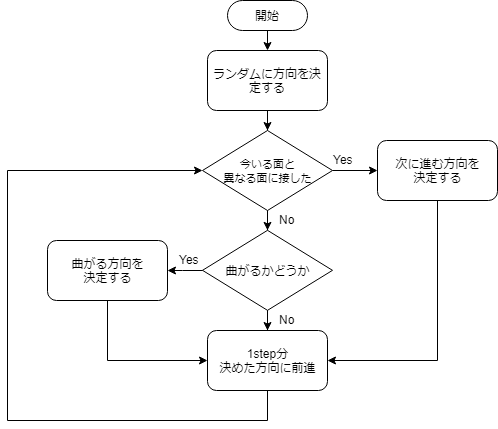
\includegraphics[width=0.7\linewidth]{png/Untitled.png}
		\caption[アルゴリズムのフローチャート]{制御されていないサイボーグインセクトのアルゴリズムのフローチャート}
		\label{fig:algorithm}
	\end{figure}
	
	制御をされていないサイボーグインセクトは,図\ref{fig:algorithm}のフローチャートに示されているアルゴリズムに従って行動する.
	このアルゴリズムでの1stepは0.1秒とする.
	また,文献より\cite{speed},制御されていない場合のサイボーグインセクトの速度は 60cm/s とする.
	
	\subsection{進行方向ベクトルの初期値決定}
	\label{random}
	探索が開始されたときに実行される.
	どの方向に進むのかをランダムに決定する.
	以降,サイボーグインセクトが進む方向の単位ベクトルを進行方向ベクトルと呼ぶ.
		
	\subsection{進行方向ベクトルを変更するかの判定}
	\label{carb}
	サイボーグインセクトは,1step毎に現在の進行方向ベクトルを新しい進行方向ベクトルに変更するかの判定を行う.
	この時に,進行方向ベクトルを変更する確率は1\%とする.
	
	\subsection{回転角の決定}
	現在の進行方向ベクトルからどれだけ回転するかの決定を行う.
	この時,現在の進行方向ベクトルから角度が大きく異なる進行方向ベクトルほど選択する確率が低くなるように設定した.
	これは,サイボーグインセクトが移動中に方向転換する場合において,回転角が大きい進行方向ベクトルと回転角が小さい進行方向ベクトルならば,変更にかかるエネルギーの少なさから回転角の小さいベクトルを選びやすいと考えたためである.
	また,現在接している面から別の面へ移動するようなベクトルには回転しないものとする.
	図\ref{fig:bend}のように赤い矢印であらわされるベクトルには回転する可能性が存在し,青のベクトルのように接する面が変わるベクトルには回転しないものとする.
	\begin{figure}
		\centering
		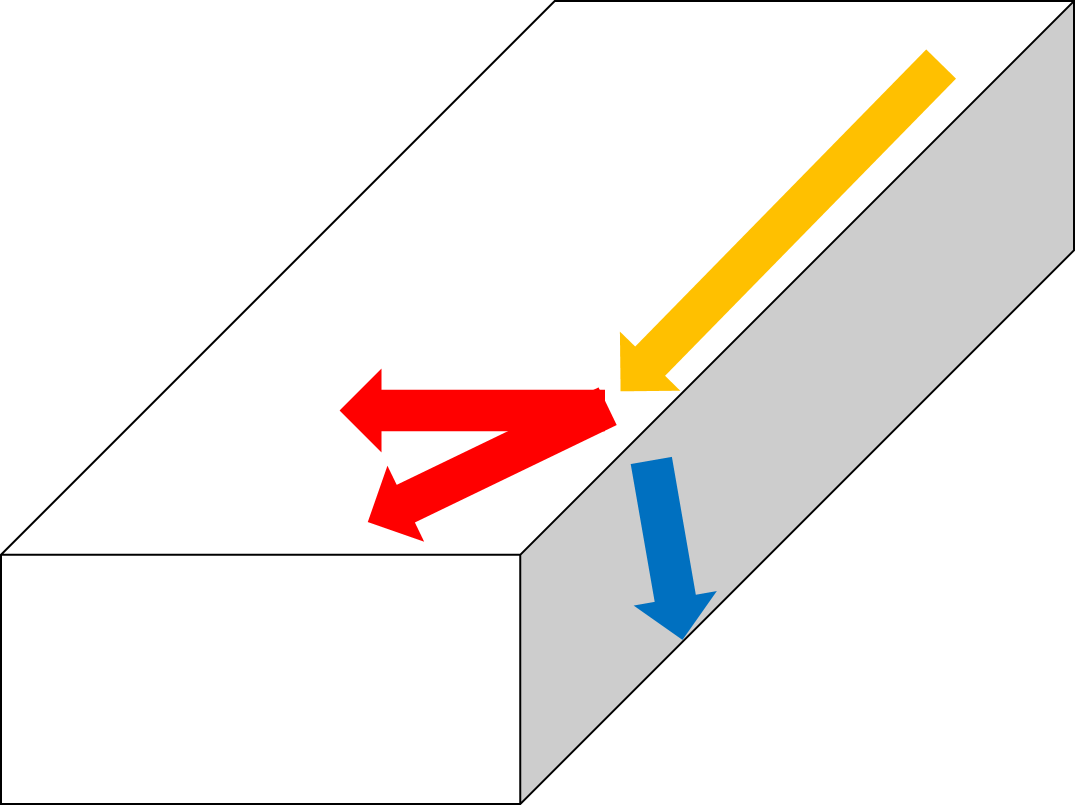
\includegraphics[width=0.35\linewidth]{png/bend.png}
		\caption[ベクトルの決定]{回転できるベクトル(赤)と回転できないベクトル(青)の例}
		\label{fig:bend}
	\end{figure}
	
	ここで,回転する角度は,平均0,分散$\frac{\pi}{6}$の正規分布に従って決定される.
	
	\subsection{1step分前進}
	サイボーグインセクトは,進行方向のベクトルに1step分前進する.
	また,途中で障害物があったり接している面が途切れたりなどで1step分の距離を進めない場合は,進めるところまで進み,その位置で停止する.
	
	\subsection{面と面が構成する境界線に接したかの判定}
	サイボーグインセクトは,現在いる場所が面と面が構成する境界線に接しているかどうかを1step毎に判定を行う.
	
	\subsection{次の進行方向ベクトルの決定}
	\label{vector}
	サイボーグインセクトは次の進行方向ベクトルを計算する.次の進行方向ベクトルの候補として,図\ref{fig:vec_surface}のような3種類のベクトルを計算する.この時,サイボーグインセクトがすでに境界線に沿って進んでいる場合は,図\ref{fig:vec_boader}のように,新しく接した境界線に沿うような2つのベクトルを計算する.
	\begin{enumerate}
		\item 境界線に平行なベクトル
		\item 境界線に平行な1.の逆ベクトル
		\item 現在の方向を保ちつつ,新しく接した面に平行なベクトル
	\end{enumerate}
	\begin{figure}
		\begin{minipage}{0.5\linewidth}
			\centering
			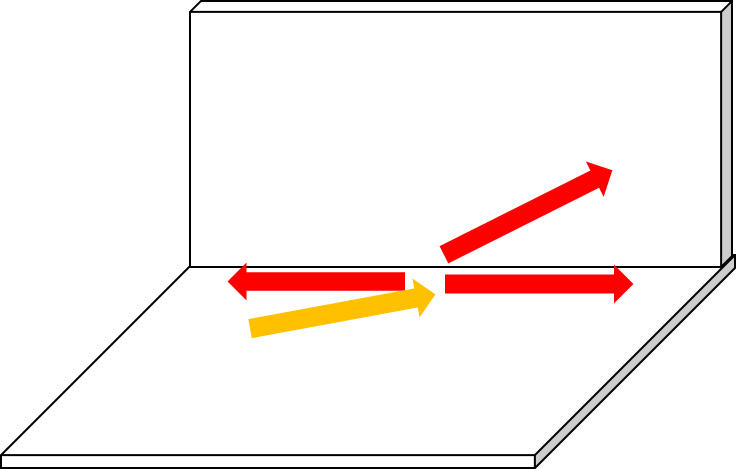
\includegraphics[width=1\linewidth]{png/vector.png}
			\subcaption{面上を進んでいる場合}\label{fig:vec_surface}
		\end{minipage}
		\begin{minipage}{0.5\linewidth}
			\centering
			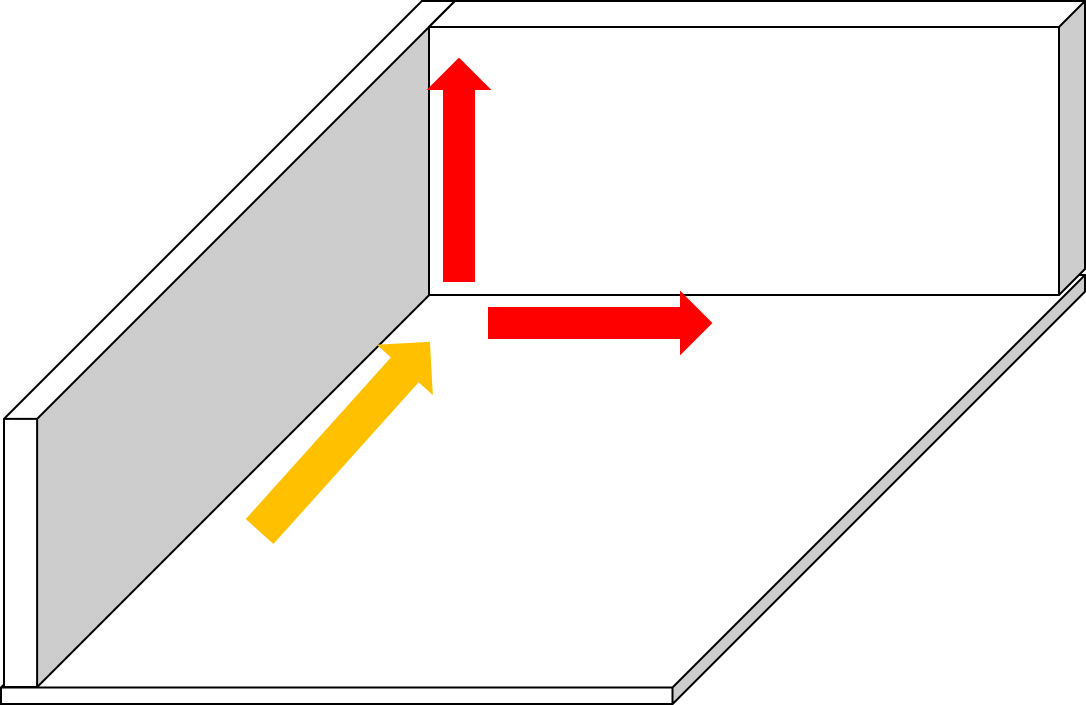
\includegraphics[width=1\linewidth]{png/vector2.png}
			\subcaption{境界線上を進んでいる場合}\label{fig:vec_boader}
		\end{minipage}\\
		\caption{次に進む方向のベクトル}
		\label{fig:vector}
	\end{figure}
	
	それぞれの具体的な計算方法は以下の章で説明する.
	\subsubsection{境界線に平行なベクトル}
	\label{boader}
	新たに接した境界線のベクトルを求めて,そのベクトルに平行な単位ベクトルを次の進行方向ベクトルの候補とする.
	図\ref{fig:vec_boader}のように境界線上を進んでいる場合,新たに接した境界線が2つあるため,その2つの境界線にそれぞれ平行な単位ベクトルを次の進行方向ベクトルの候補とする.
	
	\subsubsection{境界線に平行なベクトルの逆ベクトル}
	\ref{boader}章で求めたベクトルの逆ベクトルを次の進行方向ベクトルの候補とする.
	
	\subsubsection{現在の方向を保ちつつ,新しく接した面に平行なベクトル}
	\label{rotation}
	新たに接した境界線を軸にして,現在の進行方向ベクトルを回転することで次の進行方向ベクトルの候補を計算する.
	現在の進行方向ベクトルの境界線に垂直な成分から,新しく検知した面に平行で境界線に垂直なベクトルへ反時計回りでなす角を$ \phi $としたときに,現在の進行方向ベクトル$\vec{v}$を$\phi$だけ回転することで,次の進行方向ベクトルの候補$\vec{l}$が得られる.
	
	回転角$\phi$は図\ref{fig:xz}のように,現在の進行方向ベクトルと新たに検知した面に平行で境界線に垂直なベクトルを求めて,進行方向ベクトルの垂直成分から求めたベクトルへ反時計回りになす角である.
	
	\begin{figure}
		\begin{minipage}{0.5\linewidth}
			\centering
			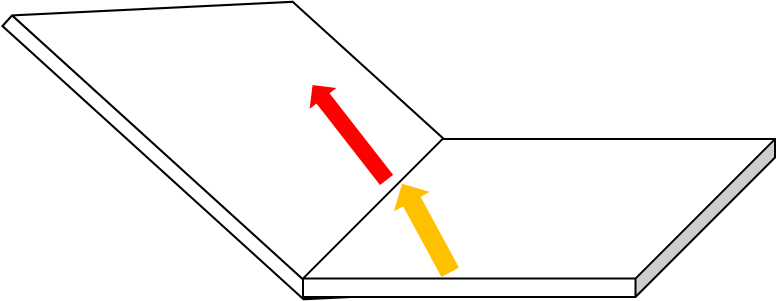
\includegraphics[width=1\linewidth]{png/sub.png}
			\subcaption{現在のベクトルと求めるベクトル}
			\label{fig:phi}
		\end{minipage}
		\begin{minipage}{0.5\linewidth}
			\centering
			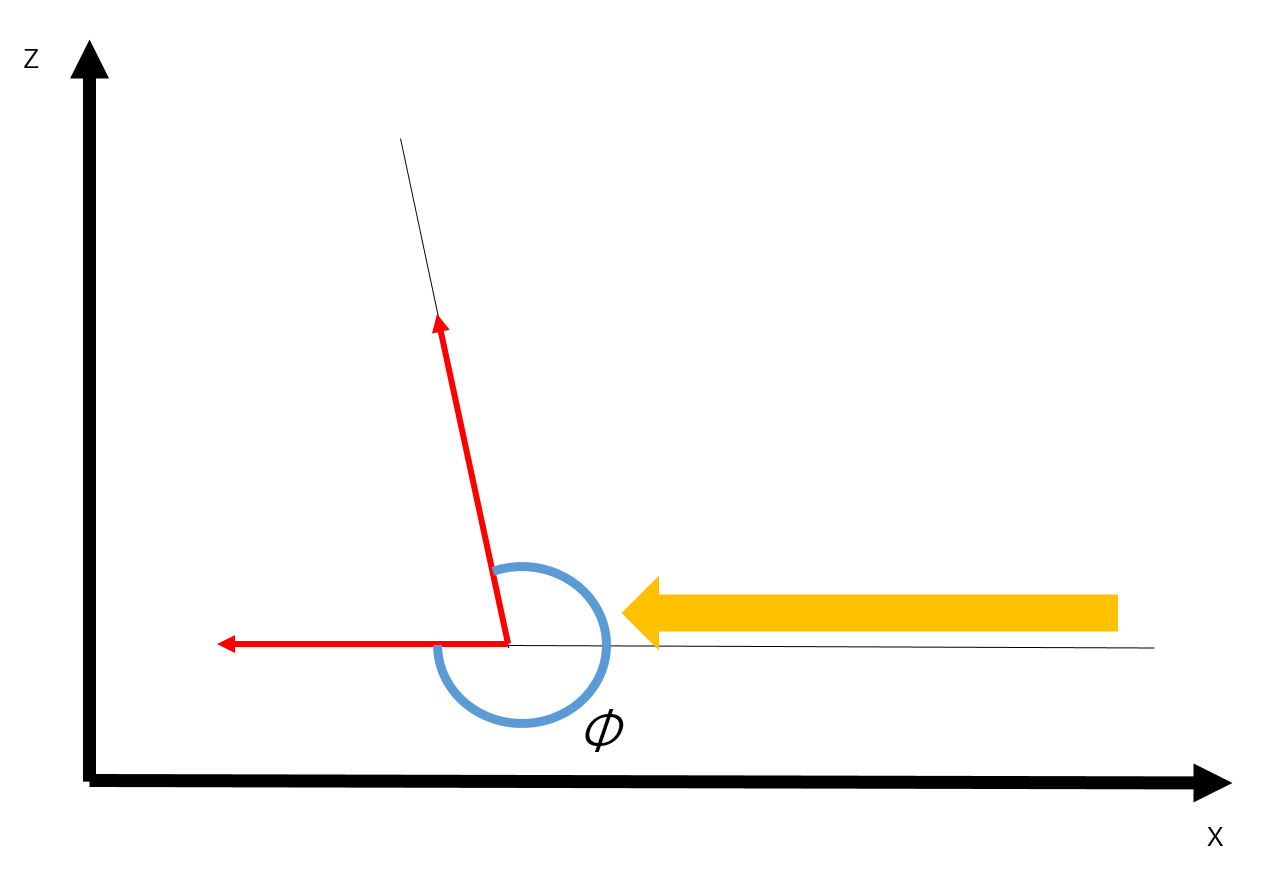
\includegraphics[width=1\linewidth]{png/rotation.png}
			\subcaption{図\ref{fig:phi}をy軸方向から見た図}
			\label{fig:xz}
		\end{minipage}
		\caption{なす角$\phi$の位置}
		\label{fig:rotation}
	\end{figure}
	
	境界線に平行なベクトルを$\vec{b} $とした際に,次の進行方向ベクトルの候補$\vec{l}$は式\ref{formula:l}によってあらわされる.
	\begin{equation}
	\label{formula:l}
	\vec{l} = R_{\vec{b}}(\phi)\vec{v}
	\end{equation}
	
	ここで$R_{\vec{b}}(\phi)$は境界線に平行なベクトル$\vec{b}$を軸に角度$\phi$だけ回転させるための回転行列とする.
	回転行列$R_{\vec{b}}(\phi)$は式\ref{formula:rotation}で計算される.
	
	\begin{equation}
	\label{formula:rotation}
	R_{\vec{b}}(\phi)=\left( \begin{array}{ccc}
	b_x^2(1-\cos\phi)+\cos\phi & b_x b_y (1-\cos\phi) - b_z\sin\phi & b_z b_x (1-\cos\phi) + b_y\sin\phi \\
	b_x b_y (1-\cos\phi)+b_z \sin\phi & b_y^2 (1-\cos\phi) + \cos\phi & b_y b_z (1-\cos\phi) - b_x\sin\phi \\
	b_z b_x (1-\cos\phi)- b_y\sin\phi & b_y b_z (1-\cos\phi) + b_x \sin\phi & b_z^2 (1-\cos\phi) + \cos\phi \\
	\end{array} \right)
	\end{equation}
	
	\subsubsection{ベクトルの決定}
	\ref{boader}章から\ref{rotation}章で計算したベクトル$\vec{l}_i$から,次の進行方向ベクトルを決定する.
	次の進行方向ベクトルは,基準ベクトルとの差異による確率に従って決定される.
	基準ベクトルは,現在の進行方向ベクトルと重力ベクトルとの和によって計算される.
	まず,現在の方向ベクトル$ \vec{v} $と重力ベクトル$ \vec{g} $から基準となるベクトル$ \vec{a} $を計算する式は以下の通りである.
	\begin{equation}
	\vec{m} = \vec{v} +\frac{49}{60} \vec{g} 
	\end{equation}

	\begin{equation}
		\vec{a} = \frac{\vec{m}}{|\vec{m}|}
	\end{equation}
	ここで,$ \vec{g} $の係数は,0.1秒分の自由落下の計算から求めている.また,単位ベクトルである$\vec{l}_i$と合わせるために$\vec{a}$も単位ベクトルとなるように求めている.
	
	次に,各ベクトルを選択する確率は式\ref{formula:prob}によって計算される.
	\begin{equation}
	\label{formula:prob}
	P(\vec{l}_i) = \frac{1}{n-1}(1 - \frac{|\vec{a} - \vec{l}_i |}{\sum_{k=1}^{n}|\vec{a} - \vec{l}_k|})
	\end{equation}
	
	ここで,$ \vec{l}_i $は\ref{boader}章から\ref{rotation}章で計算した次の進行方向ベクトルの候補で,$ i = (1, .. ,n) $である.
	
	\section{制御モデル}
	\label{sec:control}
	この章では,\ref{sec:algorithm}章で説明したサイボーグインセクトのモデルへの制御を説明する.
	
	この制御の目的は,空間全体の探索にかかる時間を短縮することである.
	また,サイボーグインセクトへの負担や消費電力の軽減のため,サイボーグインセクトに対して常に制御を行うのではなくある周期ごとに断続な制御を与える.
	
	文献\cite{exploration}のフロッキングによる空間探索の手法と同様に,探索の冗長性を小さくすることで探索にかかる時間の軽減されると一般的に言うことができる.
	そこで,複数のサイボーグインセクトが同一の領域を探索することがないように,フロッキングの衝突回避のアルゴリズムを応用する.
	また,本研究でサイボーグインセクトに用いると仮定しているマダガスカルゴキブリは,一般的に障害物に沿って移動することが知られている.
	同様の場所を繰り返し移動することで,探索が冗長になってしまう可能性があると考えられる.
	よって,壁に沿って移動している場合は壁から離れさせるような制御を行うことで,探索にかかる時間の軽減を目指す.
	
	制御を加える場合の全体のアルゴリズムは図\ref{fig:control}のフローチャートであらわされる.
	
	\begin{figure}
		\centering
		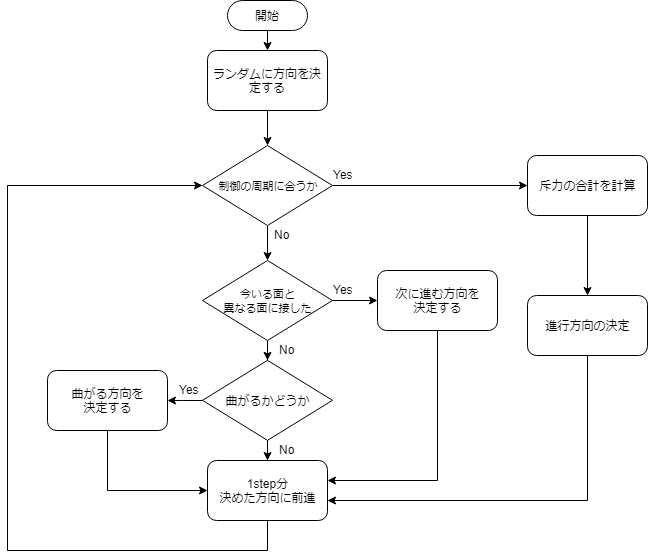
\includegraphics[width=0.8\linewidth]{png/control.png}
		\caption[アルゴリズムのフローチャート]{サイボーグインセクトを制御する場合のアルゴリズムのフローチャート}
		\label{fig:control}
	\end{figure}
	ここでの制御の周期Tはシミュレーションを行う際のパラメータとする.
	
	\subsection{斥力の合計を計算}
	\label{sec:repulsive}
	あるサイボーグインセクトに対して,距離の近いサイボーグインセクトと障害物から斥力が働くとして考え,その斥力の合計を計算する\cite{flocking-robot}.
	
	\subsubsection{サイボーグインセクトからの斥力}
	\label{sec:repulsive_insect}
	まず,周囲のサイボーグインセクトと通信を行い,通信距離内にサイボーグインセクトがいるかどうかを確認する.
	自身の通信距離内にサイボーグインセクトがいた場合,次のようにして斥力を求める.
	座標$(x,y,z)$にいるサイボーグインセクトが,座標$(x_a,y_a,z_a)$にいるサイボーグインセクト$a$から受ける斥力$\vec{f}_a$は式\ref{formula:f_a}で求められる.
	この式\ref{formula:f_a}は,文献\cite{steering}の衝突回避の式を参考にした.近い場合はさらに大きな斥力を持たせたかったため,正規化したのちに$d_a^2$で割るというように変更した.
	\begin{equation}
	\label{formula:f_a}
	\vec{f}_a = (\frac{x - x_a}{d_a^2},\frac{y- y_a}{d_a^2},\frac{z - z_a}{d_a^2})
	\end{equation}
	
	個体$a$との距離は式\ref{formula:distance}により求められる.また,この時の距離$d_a$は通信可能距離である5mを1とするような正規化を行う.
	\begin{equation}
	\label{formula:distance}
	d_a = \sqrt{(x-x_a)^2+(y-y_a)^2+(z-z_a)^2}
	\end{equation}
	
	また,通信距離内にいるサイボーグインセクトが複数存在する場合は,以下の式で斥力の合計を計算する.ここで,$A$は通信距離内にいるサイボーグインセクトの集合とする.
	\begin{equation}
	\vec{F}_A = \sum_{k \in A}\vec{f}_k
	\label{formula:repalsive}
	\end{equation}
	
	\subsubsection{障害物からの斥力}
	\label{sec:repulsive_object}
	この制御は,距離$r$以内にある障害物から斥力を計算することで実現する.ここでは,今自分がいる面からは斥力は受けないものとして考える.
	
	この場合の斥力を求める式は式\ref{formula:wall}となる.また,この時の距離$d_o$はパラメータ$r$で正規化を行う.
	この式\ref{formula:wall}も式\ref{formula:f_a}と同様に,文献\cite{steering}の衝突回避の式を参考にして考案した.
	式\ref{formula:f_a}以上に近くにある障害物からの斥力を大きくしたかったため,$d_o^3$で割ることにした.
	
	\begin{equation}
	\vec{o} =  (\frac{x - x_o}{d_o^3},\frac{y- y_o}{d_o^3},\frac{z - z_o}{d_o^3})
	\label{formula:wall}
	\end{equation}
	
	\begin{equation}
	\label{formula:distance_object}
	d_o = \sqrt{(x-x_o)^2+(y-y_o)^2+(z-z_o)^2}	
	\end{equation}
	
	また,周囲の障害物からサイボーグインセクトにかかる斥力の合計は以下の式であらわされる.
	
	\begin{equation}
	\vec{F}_o = \sum_{k \in O}\vec{o}_k
	\label{formula:repalsive_object}
	\end{equation}
	
	$O$はサイボーグインセクトから距離$r$以内にある障害物の集合である.
	
	\subsubsection{斥力の合計}
	\ref{sec:repulsive_insect}章と\ref{sec:repulsive_object}章で求められる斥力を足すことで,ある個体にかかる斥力の和が計算される.よって,斥力$\vec{F}$は$\alpha$をパラメータとして式\ref{formula:repulsive_sum}であらわされる.
	\begin{equation}
	\vec{F} = \alpha\vec{F}_A + (1 - \alpha)\vec{F}_o
	\label{formula:repulsive_sum}
	\end{equation}
	
	
	\subsection{進行方向の決定}
	\label{sec:decide}
	計算した斥力から次の進行方向ベクトルを決定する.
	
	\ref{sec:repulsive}章で計算した斥力が今いる面に対して垂直な成分を持っている場合は,今いる面に射影したベクトルを次の進行方向ベクトルとする.
	図\ref{fig:repulsive}の赤い矢印が他のサイボーグインセクトや障害物から受ける斥力の合計とした場合,今いる面に平行な単位ベクトルである黄色の矢印が実際に決定される進行方向ベクトルとなる.
	\begin{figure}
		\centering
		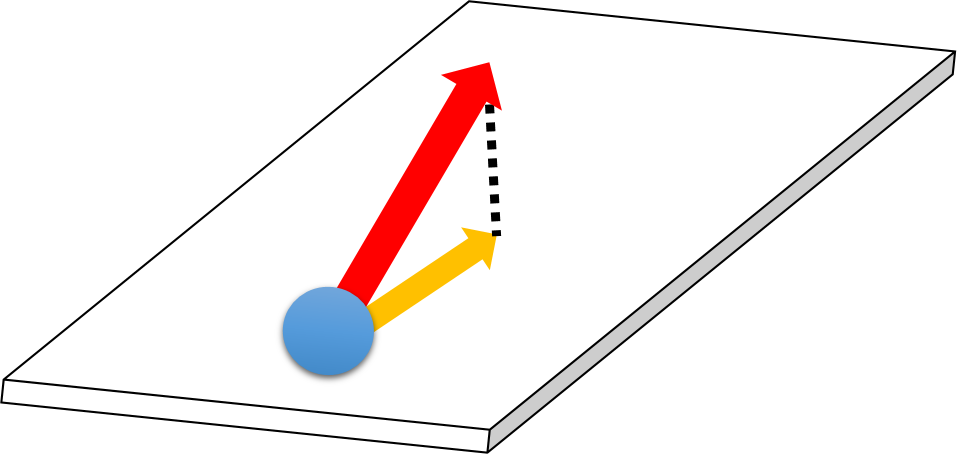
\includegraphics[width=0.35\linewidth]{png/repulsive.png}
		\caption[斥力の射影]{斥力の合計と決定した進行方向ベクトル}
		\label{fig:repulsive}
	\end{figure}
	
	\subsection{パラメータ設定}
	この章では,サイボーグインセクトを制御する場合に考えられるパラメータの設定を決定した.
	
	制御に関するパラメータとして,表\ref{tab:para}の3つを設定する.
	
	\begin{table}
		\centering
		\caption{制御に関するパラメータ}
		\label{tab:para}
		\begin{tabular}{|c|c|}
			\hline
			T(step) & 制御を行う周期 \\ \hline
			r(m) & 障害物から斥力を受ける最大距離 \\ \hline
			$\alpha$ & 斥力を合計するときの重み \\ \hline
		\end{tabular}
	\end{table}

	$r$は,壁沿いに動くことが多いことを理由として障害物からの斥力を設定しているため,大きい値である必要はないと考えた.そこで,壁から0.2mを基準とすることにした.
	$\alpha$は,$r$と関係していると考えられる.サイボーグインセクト同士の探索領域が重ならないようにするには,サイボーグインセクト同士の距離が4m以上である必要がある.そこで,壁から離れる制御とサイボーグインセクト同士が離れる制御に関して,壁沿いに動いている状態で,壁の逆側4mの距離にサイボーグインセクト1匹がいる場合は斥力が釣り合ってほしいと考えた.よって,$\alpha$は$r = 0.2$の場合に釣り合うように設定を行い,$\alpha = 0.6$とすることにした.
	
	また,以上のパラメータを設定した場合に$T$を変化させながら実験を行い探索率の推移を比較する.$T$は,100,500,1000と変化させる.
	\section{実験結果}
	\label{sec:result}
	
	この章では,\ref{sec:algorithm}章と\ref{sec:control}章で述べたサイボーグインセクトのモデルを使ったシミュレーションの結果を示す.
	
	\subsection{1匹のサイボーグインセクトが行う空間探索}
	この章では,\ref{sec:algorithm}章で記述したアルゴリズムに従うサイボーグインセクト1匹が空間を探索する様子を確認した.
	シミュレーションのパラメータは表\ref{tab:ex}のように設定した.探索する空間の広さは,サイボーグインセクト100匹で探索しようと考えている空間の100分の1の広さに決定した.
	
	\begin{table}
		\centering
		\label{tab:ex}
		\caption{1匹で探索する場合のシミュレーションのパラメータ}
		\begin{tabular}{|c|c|}
			\hline
			空間の広さ & 8m $\times$ 15m $\times$ 4m \\ \hline
			ボクセルサイズ & 10cm \\ \hline
			障害物の占有率 & 60\% \\ \hline
						N & 1匹 \\ \hline
		\end{tabular}
	\end{table}
	
	図\ref{fig:1_finish}にサイボーグインセクト1匹が空間探索を終えた時のマップの様子を示した.
	
	\begin{figure}
		\begin{minipage}{0.5\linewidth}
			\centering
			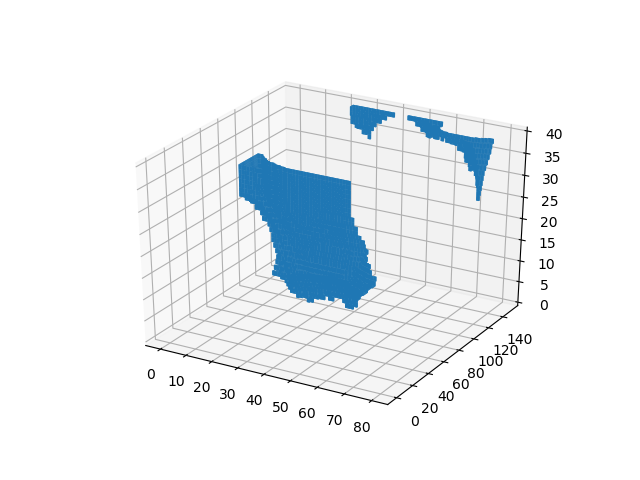
\includegraphics[width=1\linewidth]{png/Figure_49500.png}
			\subcaption{1回目}
			\label{fig:1-1}
		\end{minipage}
		\begin{minipage}{0.5\linewidth}
			\centering
			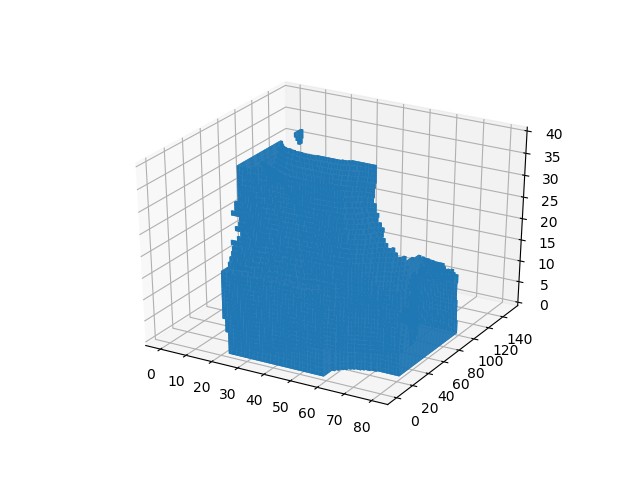
\includegraphics[width=1\linewidth]{png/Figure1_3_51000.png}
			\subcaption{2回目}
			\label{fig:1-2}
		\end{minipage}\\
		\begin{minipage}{0.5\linewidth}
			\centering
			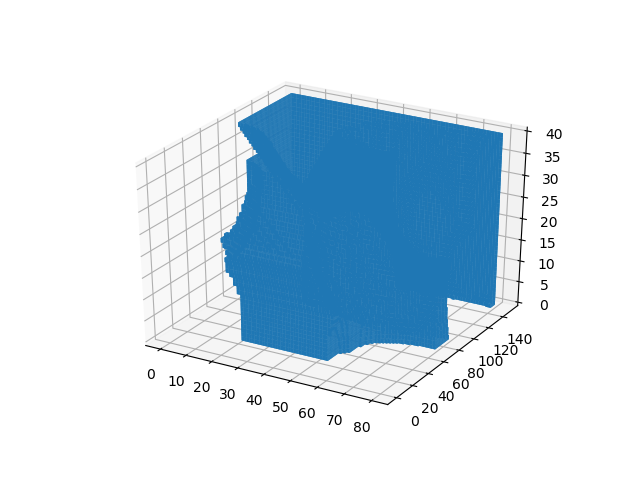
\includegraphics[width=1\linewidth]{png/Figure1_4_41000.png}
			\subcaption{3回目}
			\label{fig:1-3}
		\end{minipage}
		\begin{minipage}{0.5\linewidth}
			\centering
			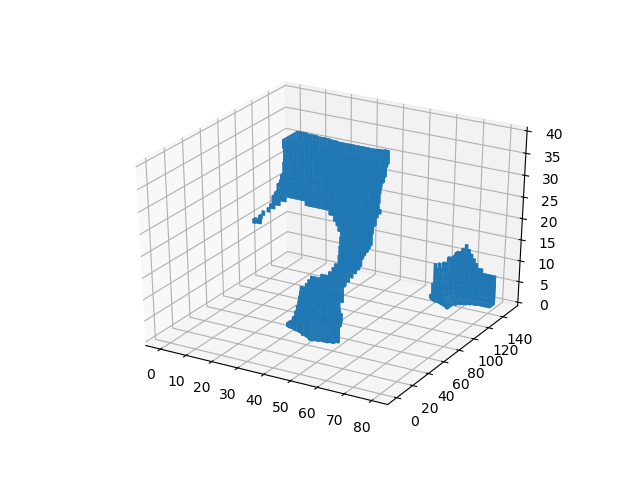
\includegraphics[width=1\linewidth]{png/Figure1_height_60000.png}
			\subcaption{4回目}
			\label{fig:1-4}
		\end{minipage}
		\caption{1匹のサイボーグインセクトが空間探索した後のマップ}
		\label{fig:1_finish}
	\end{figure}
	
	空間探索を終える条件は,すべてのボクセルが探索済みになるか,6000stepの間新しいボクセルが探索されなかったときとしている.
	ここで空間探索率は,全ボクセルに対する探索し終えたボクセルの割合として,それぞれの空間探索率と探索終了までにかかった時間を表\ref{tab:step}に示す.
	
	\begin{table}
		\centering
		\caption{探索終了時の探索率とstep数}
		\begin{tabular}{|c||c|c|}
			\hline
			 & step数 & 探索率 \\ \hline \hline
			1回目 & 49532 & 98.7\% \\ \hline
			2回目 & 51021 & 87.4\% \\ \hline
			3回目 & 41930 & 73.4\% \\ \hline
			4回目 & 62454 & 97.7\% \\ \hline
			平均 & 51234.25 & 90.875\% \\ \hline
		\end{tabular}
		\label{tab:step}
	\end{table}	
	
	探索率の平均が90.875\%であることは被災者探索を目的に考えると十分高いとは言えない.
	なぜなら,探索できていない約10\%の体積を具体的な数値で表すと,8m$\times$1.5m$\times$4m程度の大きさとなり,被災者がその中にいることが十分に考えられるためである.
	実験結果より1匹の探索では不十分であることが分かったため,\ref{sec:multi}章で複数のサイボーグインセクトでの空間探索について実験を行った.
	\subsection{複数のサイボーグインセクトが行う空間探索}
	\label{sec:multi}
	まず,シミュレーションにおいて想定している環境の説明を行う.
	今回行うシミュレーションは,地震等の自然災害で倒壊した工場のような建物から被災者をサイボーグインセクトを用いて探索するシナリオを想定している.
	経済産業省の工場立地動向調査平成29年度より,工場立地面積の平均が1228haだったため,探索する空間は崩れた工場を想定して,80m$\times$150m$\times$4mの直方体を考える.
	また,工場内を占める障害物は,文献\cite{rubble}より,形状は柱状,箱状,板状の3種類として,空間を占有する割合は60\%とする.
	
	まず,このシミュレーションで使用したパラメータを表\ref{tab:simu}に示す.また,シミュレーション上の空間はボクセルベースとなっている.
	\begin{table}
		\centering
		\caption{シミュレーションのパラメータ}
		\begin{tabular}{|c|c|}
			\hline
			空間の広さ & 80m $\times$ 150m $\times$ 4m\\ \hline
			ボクセルサイズ & 1辺10cm \\ \hline
			障害物の空間占有率 & 60\% \\ \hline
			N & 100匹 \\ \hline
			r & 0.2m \\ \hline
			$\alpha$ & 0.6 \\ \hline
		\end{tabular}
	\label{tab:simu}
	\end{table}

	この空間を探索した時の探索したボクセルの数の推移を$T$の数を変更して描画した.
	\begin{figure}
		\centering
		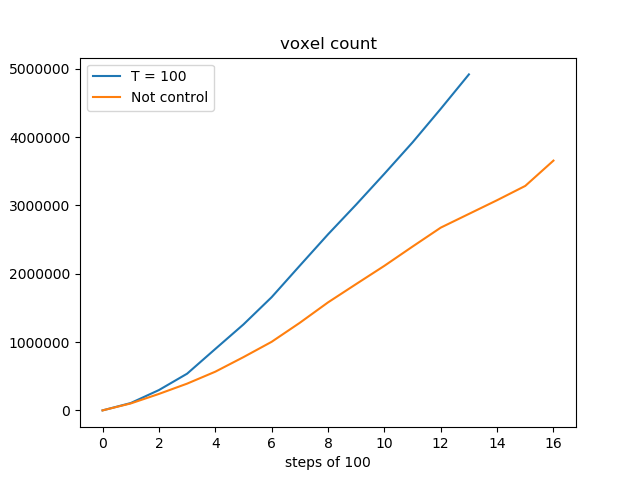
\includegraphics[width=0.8\linewidth]{png/graph_voxel-alt.png}
		\caption[実験結果]{実験結果}
		\label{fig:graph_voxel}
	\end{figure}
	図\ref{fig:graph_voxel}より,$T = 100$の場合に,Not control の時に比べると同じstep数において多くのボクセルを探索できていることがわかる.
	100stepを超えたあたりから差が付き始めているとこから,この探索したボクセル数の差は,\ref{sec:control}章の制御によって探索の冗長性がなくなっていることが理由ではないかと考えられる.
	
	\section{おわりに}
	\label{sec:last}
	本報告では,サイボーグインセクトのモデルを作成し,そのモデルにおいて迅速な被災者探索を目的としたサイボーグインセクト群への自律型制御手法の提案・評価を行った.その結果,断続的な制御であっても探索の冗長性を軽減し,探索にかかる時間を短くすることができることが分かった.
	
	今後の課題として,今回用いたシミュレーションでは空間をボクセルベースで実装しているため,より現実的な倒壊した建物内の状況で提案手法が有用であるのかの調査を行う必要がある.

%	\bibliographystyle{unsrt}
%	\bibliography{document}
	\begin{thebibliography}{99}
		%%%%%%%%%%%%%%%%%%%%%
		% 参考文献リスト
		%%%%%%%%%%%%%%%%%%%%%
		\bibitem{USR} Wen-Ta Chiu,Jeffrey arnold,Yaw-Tang Shih,Kuang-Hua Hsiung,Hsueh-Yun Chi,Chia-Huei Chiu,Wan-Chen Tsai,and William C.Huang. A Survey of International Urban Search-and-rescue Teams following the Ji Ji Earthquake. \textit{Disasters},vol.26,no.1,2002,pp.85-94
		\bibitem{environment}Casper J and Murphy R R. Human-robot interactions during the robot-assisted urban search and rescue response at the world trade center.\textit{Systems,Man, and Cybernetics, PartB:Cybernetics,IEEE Transactions on,33(3)},2003,367-385
		\bibitem{CyborgInsect}Alper Bozkurt,Robert F.Glimour,Ayesa Sinha,David Stern,and Amit Lal. Insect-Machine Interface Based Neurocybernetics. \textit{IEEE Trans Biomedical Eng.},vol.56,no.6,2009,pp.1727-1733
		\bibitem{CINEMa}Alper Bozkurt,Edgar Lobaton,and Mihail Sichitiu.A Biobotic Distributed Sensor Network for Under-Rubble Search and Rescue.\textit{Computer},vol.49,no.5,pp.38-46,2016
		\bibitem{flocks}Craig Reynolds. Flocks, herds and schools: A distributed behavioral model. \textit{ACM SIGGRApH Computer Graphics},vol.21,1987,pp25-34
		\bibitem{flockingsearch}M.G.C.A.Cimino,A.Lazzero,G.Vaglini. Combining stgmergic and flocking behaviors to coordinate swarms of drones performing target search. \textit{International Conference on Information,Intelligence,Systems and Applications},2015,pp.1-6
		\bibitem{steering}Craig Reynolds. Steering behaiviors for autonomous characters.In \textit{Proceedings of Game Developers Conference},pages 763-782,1999.
		\bibitem{obstacle}Ali E.Turgut,Hande Celikkanat,Fatih Gokce,and Erol Sahin. Self-organized flocking in mobile robot swarms. \textit{Swarm Intelligence},vol.2,pp97-120,2008
		\bibitem{exploration}Noury Bouraqadi,and Arnaud Doniec. Flocking-Based Multi-Robot Exploration. \textit{Conttol Architectures of Robots}.2009
		\bibitem{speed}J.M. Camhi, E.N. Johnson. HIGH-FREQUENCY STEERING MANEUVERS MEDIATED BY TACTILE CUES: ANTENNAL WALL-FOLLOWING IN THE COCKROACH. \textit{Journal of Experimental Biology},pp.631-643,1999
		\bibitem{flocking-robot}Ali E.Turgut, Hande Celikkanat, Faith Gokce, and Erol Sahin. Self-organized flocking in mobile robot swarms.
		\bibitem{rubble}小野里 雅彦, 増田 寿信, 毛利 健二, 伊達 宏昭, 田中 文基. がれき内部空間の構造分析に関する研究.\textit{図学研究},pp.45-48,2008
		
	\end{thebibliography}
\end{document}